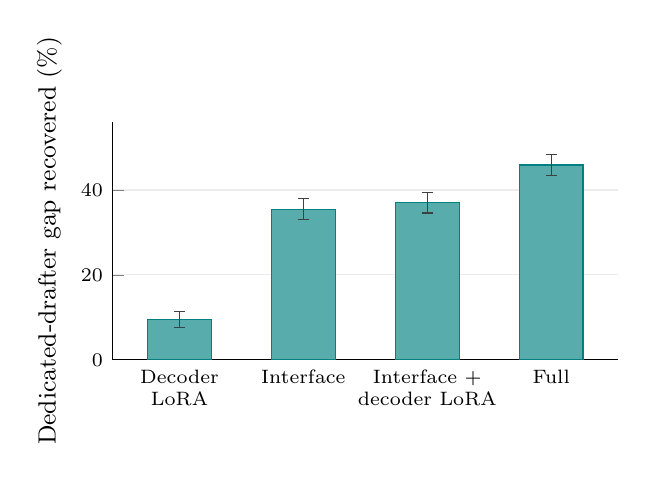
\begin{tikzpicture}
\begin{axis}[width=8.0cm,height=4.6cm,ymin=0,ymax=56,
ylabel={Dedicated-drafter gap recovered (\%)},ylabel style={font=\small},
xtick={0,1,2,3},xticklabels={Decoder\\LoRA,Interface,Interface +\\decoder LoRA,Full},
x tick label style={font=\scriptsize,align=center},tick label style={font=\scriptsize},
ymajorgrids,grid style={gray!15},axis x line*=bottom,axis y line*=left,enlarge x limits=.18]
\addplot+[ybar,mark=none,bar width=23pt,fill=teal!65,draw=teal,error bars/.cd,y dir=both,y explicit,error bar style={black!75}] coordinates {
(0,9.559455) +=(0,1.770610) -=(0,1.907351)
(1,35.499529) +=(0,2.395255) -=(0,2.401267)
(2,36.984510) +=(0,2.337847) -=(0,2.401288)
(3,45.901913) +=(0,2.418421) -=(0,2.454879)
};
\end{axis}
\end{tikzpicture}
